% This work is licensed under the Creative Commons
% Attribution-NonCommercial-ShareAlike 4.0 International License. To view a copy
% of this license, visit http://creativecommons.org/licenses/by-nc-sa/4.0/ or
% send a letter to Creative Commons, PO Box 1866, Mountain View, CA 94042, USA.

\section{Aufgabenblatt 10}
\subsection*{Aufgabe $\ast$)}
Gegeben ist der $\varepsilon$-NEA
\begin{align*}
	\A=\Big(\lbrace q_0,\ldots,q_4\rbrace,\lbrace a,b\rbrace,q_0,\Delta,\lbrace q_2\rbrace\Big)
\end{align*}

\usetikzlibrary{positioning,automata}
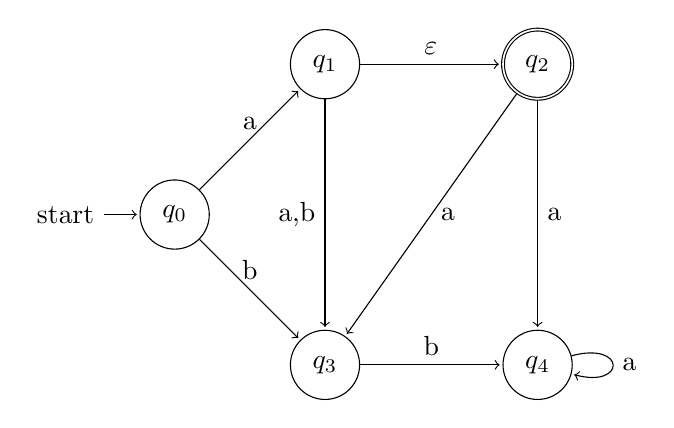
\begin{tikzpicture}[shorten >=1pt,node distance=2.7cm,on grid]
  \node[state,initial]   	(q_0)                		{$q_0$};
  \node[state] 				(q_1) [above right=of q_0] 	{$q_1$};
  \node[state, accepting] 	(q_2) [right=of q_1] 		{$q_2$};
  \node[state] 				(q_3) [below right=of q_0] 	{$q_3$};
  \node[state] 				(q_4) [right=of q_3]		{$q_4$};
  \path[->] (q_0) edge [bend left=0] node [above] {a} (q_1)
                  edge [bend left=0] node [above] {b} (q_3)
            (q_1) edge [bend left=0] node [above] {$\varepsilon$} (q_2)
            	  edge [bend left=0] node [left] {a,b} (q_3)
            (q_2) edge [bend left=0] node [right] {a} (q_3)
                  edge [bend left=0] node [right] {a} (q_4)
            (q_3) edge [bend left=0] node [above] {b} (q_4)
            (q_4) edge [loop right] node [right] {a} ();
\end{tikzpicture}

(Es fällt auf, dass $L(\A)=\lbrace a\rbrace$ ist.)
Zuerst entfernen wir die $\varepsilon$-Transitionen auf naheliegende Weise:

\usetikzlibrary{positioning,automata}
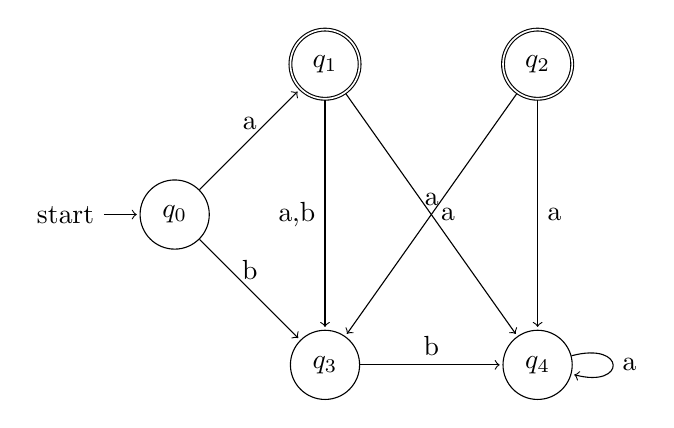
\begin{tikzpicture}[shorten >=1pt,node distance=2.7cm,on grid]
  \node[state,initial]   	(q_0)                		{$q_0$};
  \node[state, accepting]   (q_1) [above right=of q_0] 	{$q_1$};
  \node[state, accepting] 	(q_2) [right=of q_1] 		{$q_2$};
  \node[state] 				(q_3) [below right=of q_0] 	{$q_3$};
  \node[state] 				(q_4) [right=of q_3]		{$q_4$};
  \path[->] (q_0) edge [bend left=0] node [above] {a} (q_1)
                  edge [bend left=0] node [above] {b} (q_3)
            (q_1) edge [bend left=0] node [above] {a} (q_4) %Diese Transition wurde geändert
            	  edge [bend left=0] node [left] {a,b} (q_3)
            (q_2) edge [bend left=0] node [right] {a} (q_3)
                  edge [bend left=0] node [right] {a} (q_4)
            (q_3) edge [bend left=0] node [above] {b} (q_4)
            (q_4) edge [loop right] node [right] {a} ();
\end{tikzpicture}

Wichtig ist hierbei, dass nun $q_1$ auch ein Endzustand geworden ist.
Nun erzeugen wir den äquivalenten DEA mithilfe der Potenzmengenkonstruktion:

\usetikzlibrary{positioning,automata}
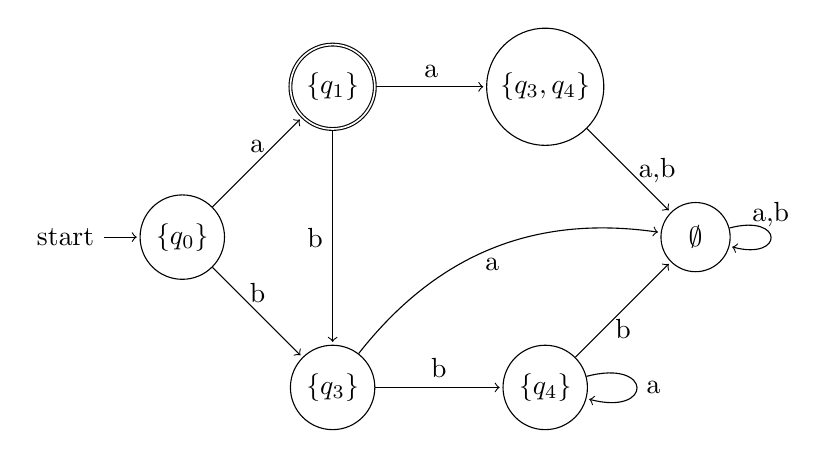
\begin{tikzpicture}[shorten >=1pt,node distance=2.7cm,on grid]
  \node[state,initial]   	(q_0)                		{$\lbrace q_0\rbrace$};
  \node[state, accepting]   (q_1) [above right=of q_0] 	{$\lbrace q_1\rbrace$};
  \node[state]			 	(q_3q_4) [right=of q_1] 		{$\lbrace q_3,q_4\rbrace$};
  \node[state] 				(q_3) [below right=of q_0] 	{$\lbrace q_3\rbrace$};
  \node[state]			 	(q_4) [right=of q_3]		{$\lbrace q_4\rbrace$};
  \node[state]				(T)	  [below right =of q_3q_4] {$\emptyset$};
  \path[->] (q_0) edge [bend left=0] node [above] {a} (q_1)
                  edge [bend left=0] node [above] {b} (q_3)
            (q_1) edge [bend left=0] node [above] {a} (q_3q_4)
            	  edge [bend left=0] node [left] {b} (q_3)
            (q_3q_4) edge [bend left=0] node [right] {a,b} (T)
                  %edge [bend left=0] node [right] {a} (q_4)
            (q_3) edge [bend left=0] node [above] {b} (q_4)
            	  edge [bend left=30] node [below] {a} (T)
            (q_4) edge [loop right] node [right] {a} ()
            	  edge [bend left=0] node [below] {b} (T)
           	(T)   edge [loop right] node [above] {a,b} ();
\end{tikzpicture}

Den unerreichbaren Zustand $q_2$ braucht man nicht beachten. Den Papierkorbzustand $\emptyset$ nicht vergessen. Also ist der äquivalente DEA:
\begin{align*}
	\A'&=\Big(\big\lbrace q_0\rbrace,\lbrace q_1\rbrace,\lbrace q_3\rbrace,\lbrace q_3,q_4\rbrace,\lbrace q_4\rbrace,\emptyset\big\rbrace,\lbrace a,b\rbrace,\lbrace q_0\rbrace,\delta,\big\lbrace\lbrace q_1\rbrace\big\rbrace\Big)\\
	\overset{\text{Umbennung}}&{=:}
	\Big(\underbrace{\lbrace p_0, p_1,p_3,p_2,p_4, p_5\rbrace}_{=:P},\lbrace a,b\rbrace,p_0,\delta,\lbrace p_1\rbrace\Big)
\end{align*}

Da $\A'$ keine unerreichbaren Zustände mehr besitzt, gilt $\A_0=\A'$.
Um $\A_{\text{red}}$ zu berechnen, berechnen wir $\sim_{\A}$ schrittweise durch $\sim_k$:
\begin{itemize}
	\item $P|_{\sim_0}=\big\lbrace\lbrace p_1\rbrace,\lbrace p_0,p_2,p_3,p_4,p_5\rbrace\big\rbrace$ (Startzustände und Endzustände trennen)
	\item $P|_{\sim_1}=\big\lbrace\lbrace p_1\rbrace,\lbrace p_0\rbrace,\lbrace p_2,p_3,p_4,p_5\rbrace\big\rbrace$
	\item $P|_{\sim_2}=\big\lbrace\lbrace p_1\rbrace,\lbrace p_0\rbrace,\lbrace p_2,p_3,p_4,p_5\rbrace\big\rbrace$
\end{itemize}
Es gilt also $\sim_2=\sim_1\implies\sim_\A=\sim_1$. 
Der Quotientenautomat
\begin{align*}
	\tilde{A}&=\big(\tilde{Q},\Sigma,\tilde{q}_0,\tilde{\delta},\tilde{F}\big)\mit\\
	\tilde{Q}&=\big\lbrace\lbrace p_1\rbrace,\lbrace p_0\rbrace,\lbrace p_2,p_3,p_4,p_5\rbrace\big\rbrace
	=
	\big\lbrace [p_1]_{\sim},[p_0]_\sim,[p_2]_\sim\big\rbrace\\
	\Sigma&=\lbrace a,b\rbrace\\
	\tilde{q}_0&=\lbrace p_0\rbrace=[p_0]_\sim\\
	\tilde{\delta}&=\left\lbrace
		\begin{array}{l}
			\big([p_0]_{\sim},a,[p_1]_{\sim}\big), \big([p_0]_{\sim},b,[p_2]_{\sim}\big),\\
			\big([p_1]_{\sim},a,[p_2]_{\sim}\big), \big([p_1]_{\sim},b,[p_2]_{\sim}\big),\\
			\big([p_2]_{\sim},a,[p_2]_{\sim}\big), \big([p_2]_{\sim},b,[p_2]_{\sim}\big)
		\end{array}
	\right\rbrace\\
	\tilde{F}&=\big\lbrace \lbrace p_1\rbrace\big\rbrace=\big\lbrace [p_1]_\sim\big\rbrace
\end{align*}
erfüllt also
\begin{align*}
	\A_{\text{red}}=\tilde{\A_0}\cong\A_0=\A'
\end{align*}
und insbesondere gilt
\begin{align*}
	L\big(\A_\red\big)=\lbrace a\rbrace.
\end{align*}

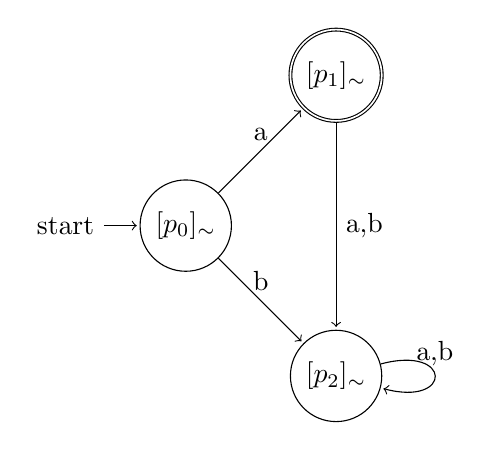
\begin{tikzpicture}[shorten >=1pt,node distance=2.7cm,on grid]
  \node[state,initial]   	(q_0)                		{$[p_0]_{\sim}$};
  \node[state, accepting]   (q_1) [above right=of q_0] 	{$[p_1]_{\sim}$};
  \node[state] 				(q_2) [below right=of q_0] 	{$[p_2]_{\sim}$};
  \path[->] (q_0) edge [bend left=0] node [above] {a} (q_1)
                  edge [bend left=0] node [above] {b} (q_2)
            (q_1) edge [bend left=0] node [right] {a,b} (q_2)
            (q_2) edge [loop right]  node [above] {a,b} ();
\end{tikzpicture}

\subsection{Aufgabe 1}
\textbf{Konvention.} Bei mir ist $\N:=\lbrace 1,2,3,\ldots\rbrace$.\nl
Meine Idee (geht sicher viel eleganter):\\
Da es sehr viele Zerlegungsmöglichkeiten pro Wort $w$ gibt, ist es geschickter zu schauen, für welche $y\in\Sigma^+$ überhaupt die Eigenschaft 
\begin{align*}
	\exists x,z\in\Sigma^\ast:\forall k\in\N:xy^kz\in L(\A)
\end{align*}
gilt.
Man sieht, dass nur $y\in\lbrace c,cd,dc\rbrace=:M$ dies erfüllen. Nun gehen wir $w$ einzeln durch und schauen uns nur die Zerlegungen an, bei der $y\in M$ gilt (denn nur die sind interessant). Da $x,z=\varepsilon$ möglich, erhalten wir genau diese möglichen Zerlegungen durch \textit{Stringvergleich}, d.h. wir schauen, ob ein $p\in M$ existiert, welches ein Substring von dem festen $w$ ist. Also: (Nutze Kurzschreibweise $\alpha|\beta|\gamma$ für Zerlegung des Wortes $w$ in $x=\alpha$, $y=\beta$ und $z=\gamma$)
\begin{itemize}
	\item $w=adc$: Mögliche Zerlegungen: 
	\begin{itemize}
		\item $ad|c|\varepsilon$: ist in $L(\A)$, aber $c$ dann nicht mehr loopbar.
		\item $a|dc|\varepsilon$: ist in $L(\A)$ und erfüllt \eqref{eqAufgabe1}.
	\end{itemize}
	\item $w=cda$ ist gar nicht in $L(\A)$, weshalb keine solche Zerlegungen existieren können, die \eqref{eqAufgabe1} erfüllen. 
	\item $w=bcdc$ Mögliche Zerlegungen: 
	\begin{itemize}
		\item $b|c|dc$: erfüllt \eqref{eqAufgabe1}.
		\item $bcd|c|\varepsilon$: erfüllt \eqref{eqAufgabe1} nicht, da $c$ nicht mehr "geloopt" werden kann, nach $acd$ gelesen wurde.
		\item $b|cd|c$: erfüllt \eqref{eqAufgabe1}.
		\item $bc|dc|\varepsilon$: erfüllt \eqref{eqAufgabe1}.
	\end{itemize}
	\item $w=acdc$ Mögliche Zerlegungen: 
	\begin{itemize}
		\item $a|c|dc$: erfüllt \eqref{eqAufgabe1}.
		\item $acd|c|\varepsilon$ erfüllt \eqref{eqAufgabe1} nicht, da $c$ dann nicht mehr geloopt werden kann.
		\item $ac|dc|\varepsilon$ erfüllt \eqref{eqAufgabe1}.
		\item $a|cd|c$ erfüllt \eqref{eqAufgabe1}.
	\end{itemize}
\end{itemize}
Somit erhalten wir für $adc$ 1, für $cda$ 0, für $bcdc$ 3 und für $acdc$ 3 Zerlegungen, die die gesuchten Eigenschaft erfüllen:

\begin{align}\label{eqAufgabe1}
	\forall k\in\N:xy^kz\in L(\A)
\end{align}

\textbf{Tutor-Lösung: (stimmt mit meiner überein)}
\begin{itemize}
	\item $w=adc\in L(\A)$: kein Zerlegung möglich bei der $y$ auch wegfallen kann
	\item $w=cda\not\in L(\A)$: keine "pumpbare" Zerlegung möglich, da nicht in der Sprache
	\item $w=bcdc\in L(\A)$:
	\begin{itemize}
		\item $x=b,\qquad,y=c,\qquad z=dc$
		\item $x=b,\qquad y=cd,\qquad z=c$
		\item $x=bc,\qquad y=dc,\qquad z=\varepsilon$
	\end{itemize}
	\item $w=acdc\in L(\A)$:
	\begin{itemize}
		\item $x=a,\qquad y=c,\qquad z=dc$
		\item $x=ac,\qquad y=dc,\qquad z=\varepsilon$
		\item $x=a,\qquad y=cd,\qquad z=\varepsilon$ 
	\end{itemize}
\end{itemize}

Beachte: falls man $0\in\N$ annimmt, entfallen noch einige Fälle oben.

\subsection{Aufgabe 2}
Die Sprache
\begin{align*}
	L:=\big\lbrace a^p\mid p\text{ ist Primzahl}\big\rbrace\mit\Sigma:=\lbrace a\rbrace
\end{align*}
ist nicht erkennbar.

\begin{proof}
	Wir führen einen Widerspruchsbeweis: Angenommen, $L$ ist erkennbar.
	Dann folgt aus dem Pumping-Lemma (3.1): Es gibt $n_0\in\N_{\geq1}$ so, dass jedes Wort $w\in L$ mit $|w|\geq n_0$ sich zerlegen lässt in $w=xyz$ mit $y\neq\varepsilon$ und $xy^kz\in L$ für alle $k\geq0$.
	Sei also $w=a\ldots a\in L$ beliebig mit $p\geq n_0$. Also gilt
	\begin{align*}
		&w=\underbrace{a\ldots a}_{p\geq n_0\text{ Stück}}\overset{!}= xy^k z\\
		&\implies \exists l,m,n\in\N_{\geq0}: w=a^p=a^l a^m a^n\\
		&\implies p=l+m+n
	\end{align*}
	Nach Voraussetzung ist $p$ eine Primzahl und nach Pumpinglemma gilt:
	\begin{align*}
		&x y^k z\in L &\forall k\in\N_{\geq0}\\
		&\implies l+m\cdot k+ n\text{ ist Primzahl} &\forall k\in\N_{\geq0}
	\end{align*}
	Dies ist aber im Allgemeinen keine Primzahl (was ich gerade leider nicht für alle Fälle zeigen kann...).\\
	Widerspruch! Somit ist $L$ nicht erkennbar.
\end{proof}

\begin{proof}[Beweis des Tutors.]\enter
	\textbf{Pumping-Lemma (vereinfacht)}:\\
	Für jede erkennbare Sprache $L$ existiert ein $n_0\in\N$ so, dass\\
	für alle Wörter $w\in L$ mit $|w|\geq n_0$\\
	existiert eine Zerlegung $w=xyz$ mit $y\neq\varepsilon$ so, dass\\
	für alle $k\in\N$ gilt: $xy^kz\in L$.\nl
	Beweis durch Widerspruch:
	Angenommen, $L$ wäre erkennbar. Dann gilt das Pumpinglemma (vereinfacht) auch für $L$.
	Sei $p$ ein Primzahl mit $p\geq n_0$ (existiert nach Satz von Euklid: Es gibt unendlich viele Primzahlen).
	Dann gilt:
	$a^p\in L$ und $|a^p|\geq n_0$.
	Damit muss es eine Zerlegung von $a^p=xyz$ geben $\rightsquigarrow x=a^n,y=a^m,z=a^{n_2}$ mit $n_1,n_2,m\in\N$ und $m>0$.
	Also gilt $p=n_1+n_2+m$. 
	Definiere $n:=n_1+n_2$.
	Da $a^p=a^{m+n}\in L$, folgt aus dem Pumping-Lemma,
	dass auch $a^{n+k\cdot m}\in L$ für alle $k\in\N$.
	Insbesondere für $k=n$ %Die Idee, die mir fehlte!
	gilt $a^{n+n\cdot m}\in L$.
	Aber falls $n\neq1$ (also $n>1$ oder $n=0$) ist $n+n\cdot m=n\cdot(m+1)$ keine Primzahl!\\
	Falls $n=1$, dann müsste $a^{n+0\cdot m}=a^n=a\in L$ gelten. Widerspruch!
\end{proof}

\subsection{Aufgabe 3}
Die Sprache
\begin{align*}
	L:=\Big\lbrace w\mid w=1^k\text{ für }k\geq0\text{ oder }w=0^j1^p\text{ für }j\geq1\text{ und }p\text{ Primzahl}\Big\rbrace\\
	\mit\Sigma=\lbrace0,1\rbrace
\end{align*}
ist nicht erkennbar.

\begin{proof}
	\textbf{Pumping-Lemma (verschärft, Änderungen unterstrichen)}:\\
	Für jede erkennbare Sprache $L$ existiert ein $n_0\in\N$ so, dass\\
	%für alle Wörter $w\in L$ mit $|w|\geq n_0$ 
	\underline{für alle Wörter $u,v,w$ mit $uvw\in L$ und $|w|\geq n_0$}\\
	existiert eine Zerlegung $\underline{v}=xyz$ mit $y\neq\varepsilon$ so, dass\\
	für alle $k\in\N$ gilt: $xy^kz\in L$.\nl
	Das vereinfachte Pumpinglemma kann hier zwar auch wieder angewendet werden, hilft uns aber nicht, da
	alle $w\in L$ mit $|w|>0$ "pumpbar" zerlegt werden können:
	\begin{itemize}
		\item $w=1^k\rightsquigarrow x=1^{k-1},y=1,z\varepsilon$
		\item $w=0^j 1^p\rightsquigarrow x=\varepsilon,y=0^j,z=1^p$
	\end{itemize}
	Es gibt also eine gültige Zerlegung, weshalb wir mit dem vereinfachten Pumpinglemma keinen Widerspruch herleiten können.
	Mit dem Pumping-Lemma in verschärfter Form kann das Ergebnis aus Aufgabe 10.2 genutzt werden:
	Sei $p$ eine Primzahl mit $p\geq n_0$. Zerlege dann das Wort $01^p$ in $u=0$, $v=1^p$ und $w=\varepsilon$.
	Es gilt $01^p\in L$ und $|v|\geq n_0$.
	Zerlege dann $v$ nun wie in 10.2 gezeigt.
\end{proof}

\subsection{Aufgabe 4}
\textbf{Satz 4.1} Ist $L$ erkennbar, so ist auch $L^\ast$ erkennbar.

\begin{proof}
	%Erinnerung: Eine Sprache $L$ ist per Definition erkennbar, wenn es einen NEA $\A$ gibt, der $L$ akzeptiert, d.a. $L=L(\A)$.\nl
	Da $L$ erkennbar ist, gibt es per Definition einen NEA
	\begin{align*}
		\A:=(Q,\Sigma,q_0,\Delta,F)
	\end{align*}
	mit $L(\A)=L$. 
	Sei nun $q_{0\varepsilon}\not\in Q$ und setze
	\begin{align*}
		\A_\varepsilon&:=\Big(Q\cup\lbrace q_{0\varepsilon}\rbrace,\Sigma,q_{0\varepsilon},\Delta_\varepsilon,\lbrace q_{0\varepsilon}\rbrace\Big)\\
		\Delta_\varepsilon&:=\Delta\cup\underbrace{\big\lbrace(f,\varepsilon,q_{0\varepsilon}):f\in F\big\rbrace}_{
			=\big(F\times\lbrace\varepsilon\rbrace\times\lbrace q_{0\varepsilon}\rbrace\big)
		}\cup\big\lbrace(q_{0\varepsilon},\varepsilon,q_{0})\big\rbrace\Big)
	\end{align*}
	
	
  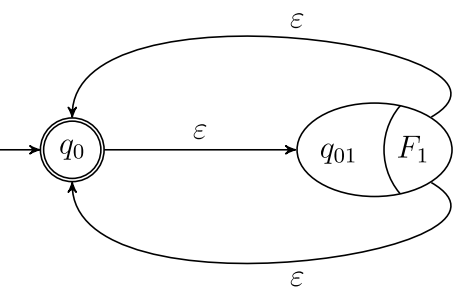
\includegraphics[width=0.7\textwidth]{pics/Blatt10_4.png}
  
  Offenbar ist $\A_\varepsilon$ ein $\varepsilon$-NEA. Mit Lemma 1.12 bekommt man einen zu $\A_\varepsilon$ äquivalenten NEA, nennen wir ihn $\A_{\text{NEA}}$. Äquivalent bedeutet $L(\A_\varepsilon)=L(\A_{\text{NEA}})$.\nl
  Bleibt noch zu zeigen, dass $L(\A_\varepsilon)=L^\ast$ gilt. 
  Sei also $w\in L^\ast$.
  Dann gibt es ein $n\in\N$ so, dass $w\in\bigcup\limits_{i=0}^n L$ ist. Man sieht leicht, dass $w\in L(\A_\varepsilon)$ liegen muss. (Das formal aufzuschreiben ist ein wenig sperrig.)
\end{proof}

\subsection{Aufgabe 5}
Folgende Automatenklassen sind in ihrer Ausdrucksstärke gleichmächtig zueinander:
NEA, $\varepsilon$-NEA (entfernen von $\varepsilon$-Transitionen), NEA mit Wortübergängen (Zwischenzustände einführen), DEA (Potenzmengenkonstruktion)\\
Transitionssysteme sind \underline{nicht} äquivalent zu obigen.\nl
Beweise oder Widerlege:
\begin{enumerate}[label=\alph*)]
	\item $L$ erkennbar $\implies\exists\varepsilon$-NEA $\A:L(\A)=L$.\\
	Stimmt, denn:
	\begin{align*}
		L\text{ erkennbar}
		\overset{\text{Def 1.6}}&\Longleftrightarrow
		\exists\text{NEA}\A_N:L(\A_N)=L\\
		\overset{\text{Lemma 10}}&\Longleftrightarrow
		\exists\varepsilon\text{-NEA }\A:L(\A)\overset{\text{Def 1.6}}{=}L(\A_N)=L
	\end{align*}
	\item $\exists$ NEA mit Wortübergängen mit $L(\A)=L\implies L$ erkennbar.\\
	Stimmt, denn:
	\begin{align*}
		&\exists\text{ NEA $\A$ mit Wortübergängen mit }L(\A)=L\\
		\overset{\text{Satz 1.9}}&\implies
		\exists\text{ NEA }\A_N:L(\A_N)\overset{\text{Def 1.6}}=L(\A)=L\\
		\overset{\text{Def 1.6}}&\implies
		L\text{ erkennbar}
	\end{align*}
	\item $\exists$ Transitionssystem $\A$ mit $L(\A)=L\implies L$ erkennbar\\
	Das stimmt nicht, Gegenbeispiel:
	\begin{align*}
		L:=\Big\lbrace a^p:p\text{ ist Primzahl }\Big\rbrace
	\end{align*}
	Transitionssystem: (wird endliche Kette, Endzustände sind Primzahlen)
	\item $L$ erkennbar und $L\subseteq L'\implies L'$ erkennbar\\
	Stimmt nicht, Gegenbeispiel:
	\begin{align*}
		L:=\lbrace aa\rbrace\qquad
		L':=\Big\lbrace a^p:p\text{ ist Primzahl }\Big\rbrace
	\end{align*}
	\item $L$ erkennbar und $L'\subseteq L\implies L'$ erkennbar.\\
	Stimmt nicht, Gegenbeispiele:
	\begin{align*}
		&L=\Big\lbrace a^n:n\in\N\big\rbrace,& l'=\big\lbrace a^p:p\text{ ist Primzahl }\Big\rbrace\\
		&L_2=\Sigma^\ast, &\Big\lbrace a^n b^n:n\in\N\Big\rbrace
	\end{align*}
	\item $L_1,L_2$ erkennbar $\implies L:=L_1\cap L_2$ erkennbar.\\
	Stimmt, wegen Satz 4.1.
	\item Wenn es ein $n\in\N$ gibt, so dass $\cong_L$ (Nerode-Rechtskongruenz) höchstens $n$ Äquivalenzklassen hat, so ist $L$ erkennbar.\\
	Ja, dies ist eine Richtung des Satzes von Myhill-Nerode
	($L$ ist erkennbar / regulär $\Longleftrightarrow \, \cong_L$ hat endlichen Index / endliche viele Äquivalenzklassen)
\end{enumerate}

